\documentclass[12pt,a4paper]{article}
\usepackage{amsmath}
\usepackage{graphicx}
\usepackage{geometry}
\usepackage{float}
\geometry{left=2.5cm,right=2.5cm,top=3cm,bottom=3cm}

\title{\textbf{Kinematic Explicit Solution and Relative Coordination Analysis}}
\author{Automated Generation System}
\date{\today}

\begin{document}
\maketitle

\section{Explicit Analytical Solution}
The degenerated planar branch is equivalent to a four-bar linkage. The original structural dimensions are first grouped into an equivalent reduced geometry, so that the scale factor is removed while the kinematic relation is preserved. In this reduced form, the linkage can be solved using the Freudenstein equation. By eliminating the coupler angle $\alpha_2$, we obtain the mathematical model based on three variable coefficients:
\begin{align}
    A(q_1) &= 2 L_{4} \left(L_{1} - L_{2} \cos{\left(q_{1} \right)}\right) \\
    B(q_1) &= - 2 L_{2} L_{4} \sin{\left(q_{1} \right)} \\
    C(q_1) &= L_{1}^{2} - 2 L_{1} L_{2} \cos{\left(q_{1} \right)} + L_{2}^{2} - L_{3}^{2} + L_{4}^{2}
\end{align}

Applying the tangent half-angle substitution, the explicit expression for the absolute rocker angle $\alpha_3$ is derived as:
\begin{equation}
    \alpha_3(q_1) = 2 \operatorname{atan}{\left(\frac{2 L_{2} L_{4} \sin{\left(q_{1} \right)} + \sqrt{4 L_{2}^{2} L_{4}^{2} \sin^{2}{\left(q_{1} \right)} + 4 L_{4}^{2} \left(L_{1} - L_{2} \cos{\left(q_{1} \right)}\right)^{2} - \left(L_{1}^{2} - 2 L_{1} L_{2} \cos{\left(q_{1} \right)} + L_{2}^{2} - L_{3}^{2} + L_{4}^{2}\right)^{2}}}{L_{1}^{2} - 2 L_{1} L_{2} \cos{\left(q_{1} \right)} + L_{2}^{2} - L_{3}^{2} + L_{4}^{2} - 2 L_{4} \left(L_{1} - L_{2} \cos{\left(q_{1} \right)}\right)} \right)}
\end{equation}

By parameterizing the linkage lengths proportionally such that the scale factor $l$ is algebraically eliminated, we substitute the relative geometry parameters $L_1=2, L_2=\sqrt{41}, L_3=5, L_4=\sqrt{41}$. The completely simplified explicit expression is:
\begin{equation}
    % 浣跨敤 resizebox 纭繚瓒呴暱鍏紡涓嶄細婧㈠嚭椤甸潰杈圭晫
    \resizebox{0.95\linewidth}{!}{$\displaystyle \alpha_3(q_1) = 2 \operatorname{atan}{\left(\frac{\sqrt{- \left(- 4 \sqrt{41} \cos{\left(q_{1} \right)} + 61\right)^{2} + 164 \left(- \sqrt{41} \cos{\left(q_{1} \right)} + 2\right)^{2} + 6724 \sin^{2}{\left(q_{1} \right)}} + 82 \sin{\left(q_{1} \right)}}{- 2 \sqrt{41} \left(- \sqrt{41} \cos{\left(q_{1} \right)} + 2\right) - 4 \sqrt{41} \cos{\left(q_{1} \right)} + 61} \right)} $}
\end{equation}

\section{Numerical Simulation}
The relative joint angles $\theta_2, \theta_4, \theta_6$ are extracted by compensating for the initial phase offsets at $q_1 = 0^\circ$. In other words, the plotted curves use the initial pose as the zero reference, so the motion starts from zero displacement rather than from the absolute joint coordinates. The resulting motion curves over a complete $360^\circ$ driving cycle are plotted in Figure \ref{fig:kinematics}.

\begin{figure}[H]
    \centering
    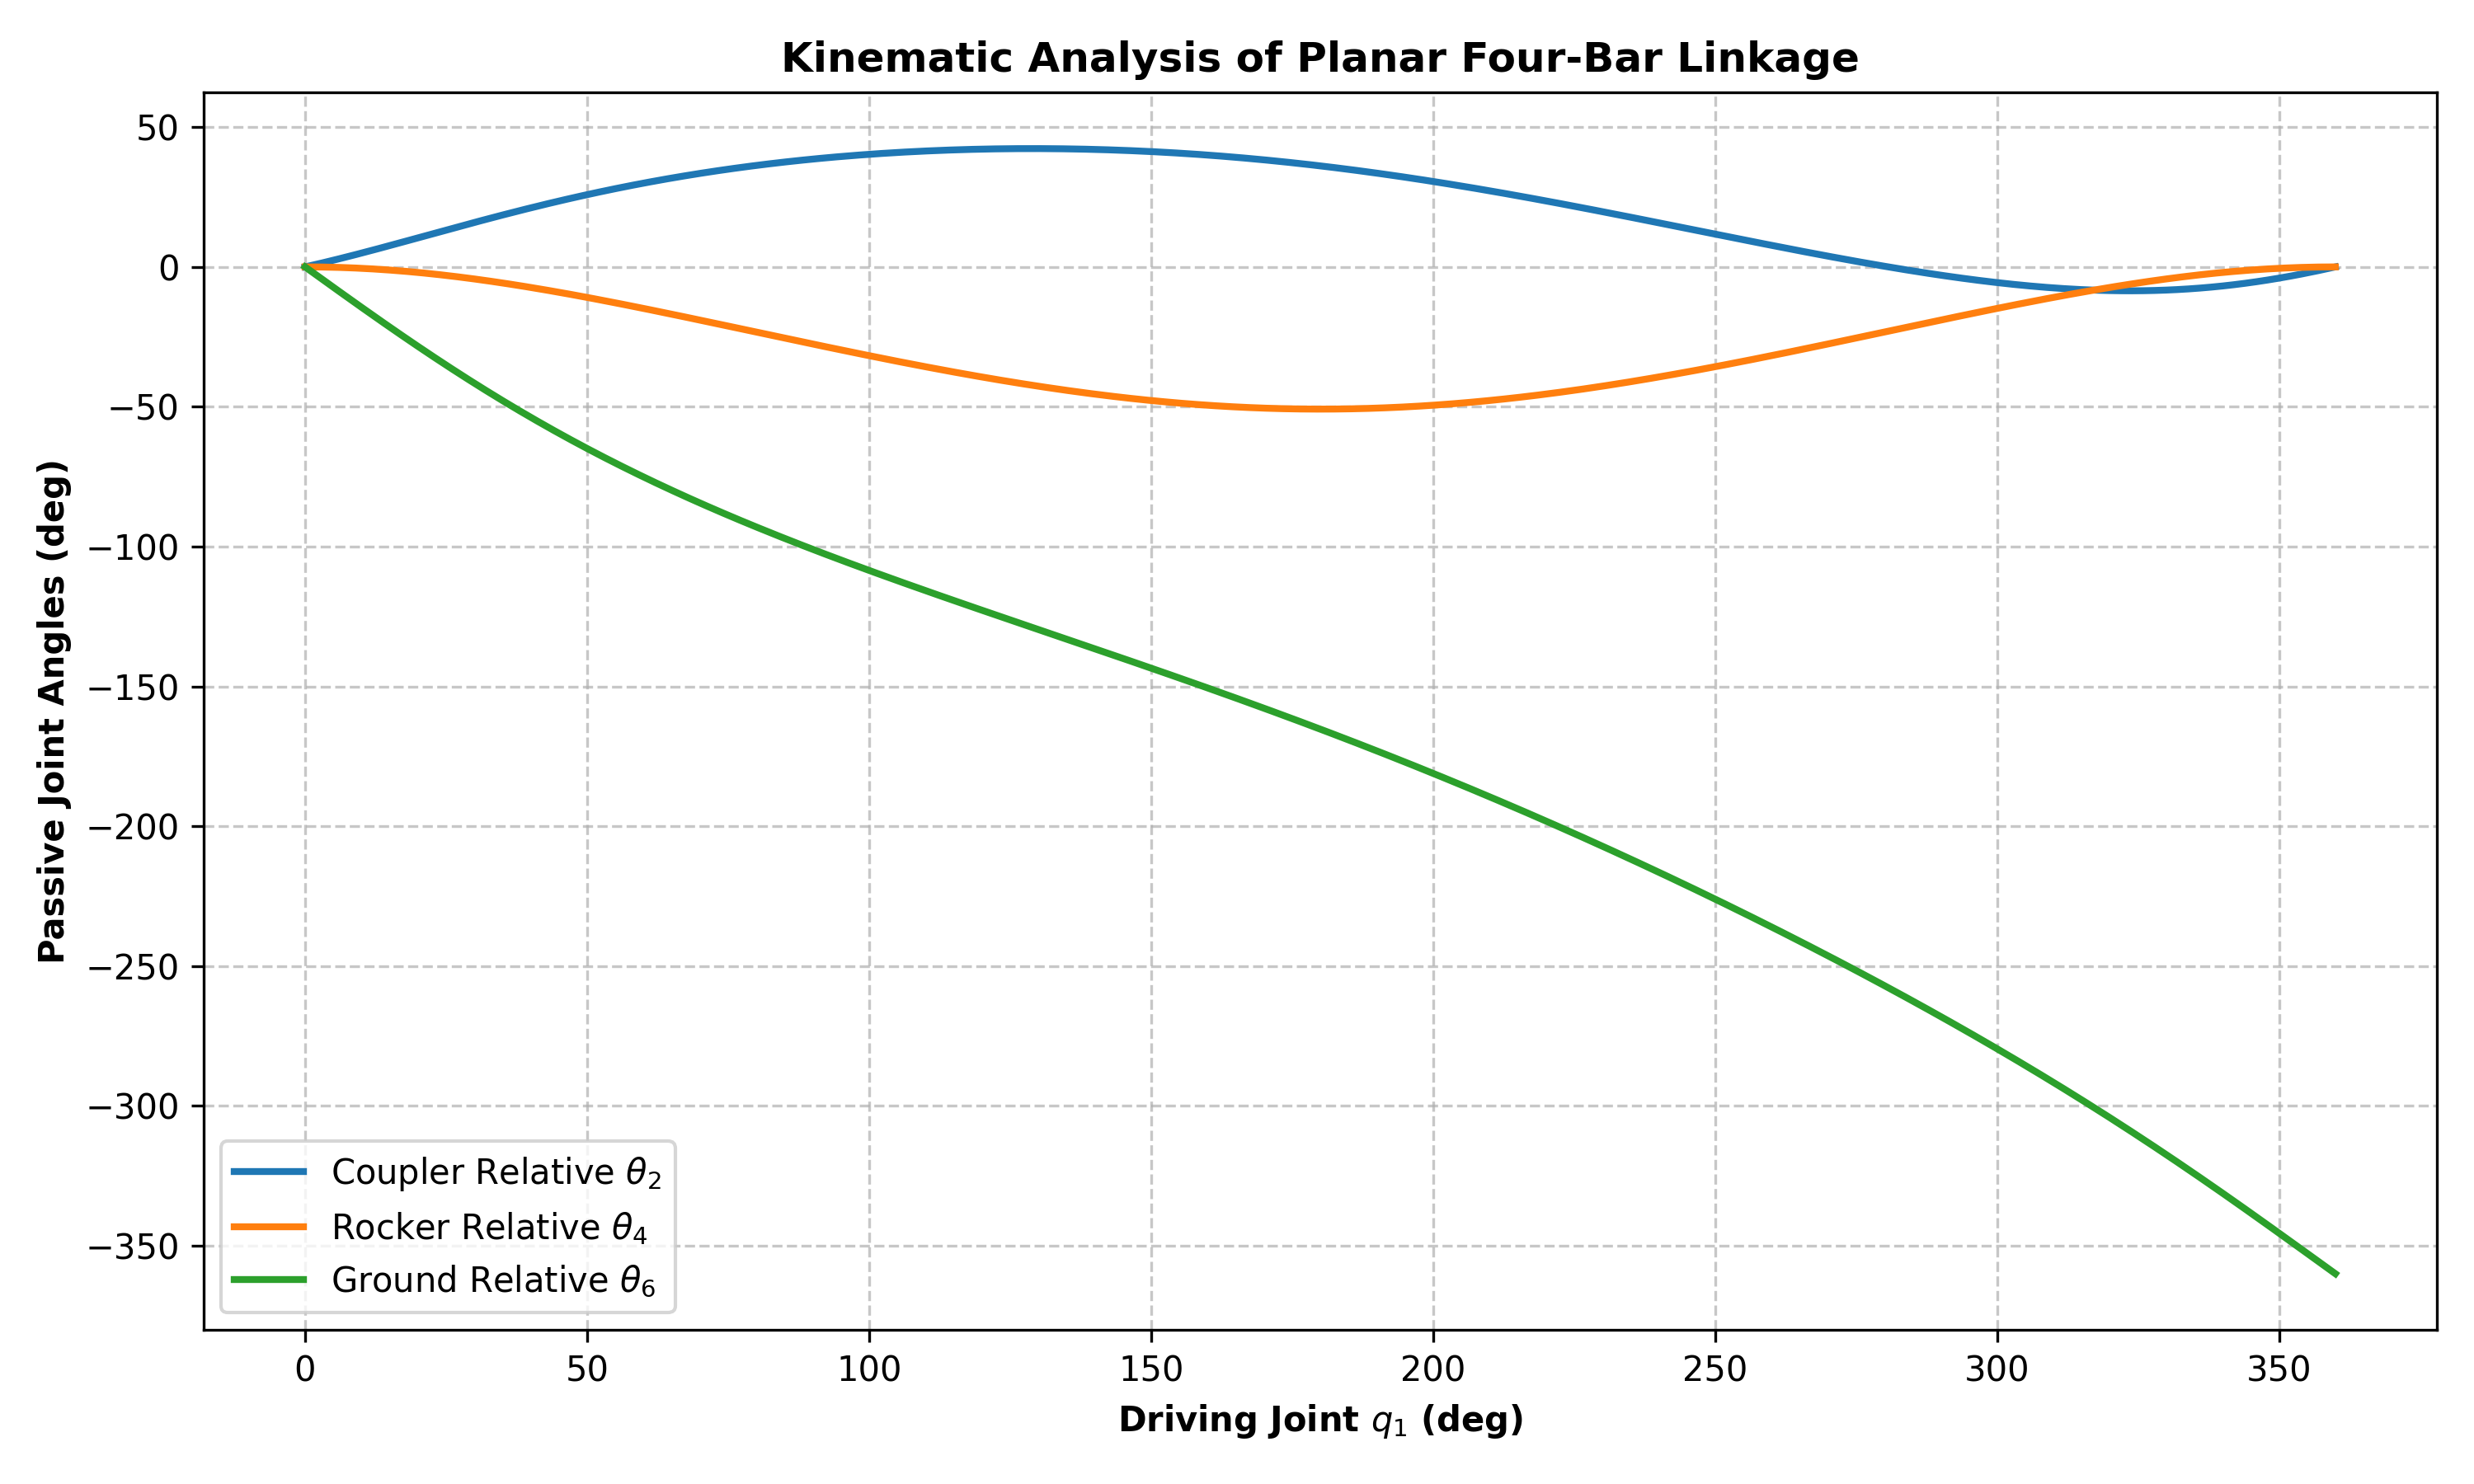
\includegraphics[width=0.9\textwidth]{kinematic_curves.png}
    \caption{Variation of passive joint angles with respect to the driving joint $q_1$.}
    \label{fig:kinematics}
\end{figure}

\end{document}

